%%%%%%%%%%%%%%% PLEASE NOTE THE FOLLOWING STYLE RESTRICTIONS %%%%%%%%%%%%%%%

%%  1. There are no new tags.  Existing LaTeX tags have been formatted to match
%%     the Preprint series style.
%%
%%  2. Do not change the margins or page size!  Do not change from the default
%%     text font!
%%
%%  3. You must use \cite in the text to mark your reference citations and
%%     \bibitem in the listing of references at the end of your chapter. See
%%     the examples in the following file. If you are using BibTeX, please
%%     supply the bst file with the manuscript file.
%%
%%  4. This macro is set up for two levels of headings (\section and
%%     \subsection). The macro will automatically number the headings for you.
%%
%%  5. No running heads are to be used for this volume.
%%
%%  6. Theorems, Lemmas, Definitions, Equations, etc. are to be double numbered,
%%     indicating the section and the occurrence of that element
%%     within that section. (For example, the first theorem in the second
%%     section would be numbered 2.1. The macro will
%%     automatically do the numbering for you.
%%
%%  7. Figures and Tables must be single-numbered.
%%     Use existing LaTeX tags for these elements.
%%     Numbering will be done automatically.
%%
%%  8. Page numbering is no longer included in this macro.
%%     Pagination will be set by the program committee.
%%
%%
%%%%%%%%%%%%%%%%%%%%%%%%%%%%%%%%%%%%%%%%%%%%%%%%%%%%%%%%%%%%%%%%%%%%%%%%%%%%%%%

\documentclass[twoside,leqno,twocolumn]{article}

% Comment out the line below if using A4 paper size
\usepackage[letterpaper]{geometry}

\usepackage{ltexpprt}
\usepackage{hyperref}

\usepackage{graphicx}

\begin{document}

%
%\newcommand\relatedversion{}
%\renewcommand\relatedversion{\thanks{The full version of the paper can be accessed at \protect\url{https://arxiv.org/abs/1902.09310}}} % Replace URL with link to full paper or comment out this line

\newcommand{\FMshop}{\textsc{finch}}

%\setcounter{chapter}{2} % If you are doing your chapter as chapter one,
%\setcounter{section}{3} % comment these two lines out.

\title{\Large \FMshop: Domain Specific Language and Code Generation for Finite Element and Finite Volume in Julia}
\author{Eric Heisler, Hari Sundar}

\date{}

\maketitle

% Copyright Statement
% When submitting your final paper to a SIAM proceedings, it is requested that you include
% the appropriate copyright in the footer of the paper.  The copyright added should be
% consistent with the copyright selected on the copyright form submitted with the paper.
% Please note that "20XX" should be changed to the year of the meeting.

% Default Copyright Statement
%\fancyfoot[R]{\scriptsize{Copyright \textcopyright\ 2022 by SIAM\\
%Unauthorized reproduction of this article is prohibited}}

% Depending on which copyright you agree to when you sign the copyright form, the copyright
% can be changed to one of the following after commenting out the default copyright statement
% above.

%\fancyfoot[R]{\scriptsize{Copyright \textcopyright\ 20XX\\
%Copyright for this paper is retained by authors}}

%\fancyfoot[R]{\scriptsize{Copyright \textcopyright\ 20XX\\
%Copyright retained by principal author's organization}}

%\pagenumbering{arabic}
%\setcounter{page}{1}%Leave this line commented out.

\begin{abstract} \small\baselineskip=9pt 
We introduce \FMshop, a Julia-based domain specific language (DSL) for solving partial differential equations using the finite element and finite volume methods. A key focus of the framework is code generation for either internal numerical solvers or external targets. Internal options use a modular set of solvers written in Julia to provide a direct, real-time solution from within the DSL itself. In contrast, the external code generation produces a set of code files that can be compiled or run in an external context such as Matlab, for smaller problems or prototypes, or the \texttt{C++} and \texttt{MPI} based framework \textsc{Dendro} for large-scale problems needing scalability. By generating code for external targets, we are able to take advantage of their capabilities without needlessly duplicating them, and provide a range of solutions tailored to the specific problem or the needs of the domain scientist. The modular design of \FMshop\ allows the ongoing development of these target modules resulting an a more extensible framework and a broader set of suitable applications. The inclusion of both finite element and finite volume methods also contributes to this goal. Another focus is on complex systems containing many PDEs that could be challenging to code and optimize by hand, but are relatively simple to specify using the DSL. In this paper we present the key features of \FMshop that set it apart from many other DSL options, outline the current capabilities as well as several that are under development, and present some examples of it in action.
\end{abstract}

\section{Introduction}
Solving partial differential equations(PDEs) numerically on a large scale involves a compromise between highly optimized code that exploits details of the problem and hardware to build the most efficient solution, and extensible code that can be adapted to variations in the problem and the computing environment. Rapidly evolving technology and a shift to heterogeneous systems places a higher value on the latter, prompting a move away from hand-written code made by experts in high performance computing, to generated code produced through a high-level domain specific language (DSL). Another factor in this change is the realm of medium-scale problems where the cost of developing optimal code may not be justified. At this scale it is up to domain scientists to develop their own software or piece it together from more general-purpose libraries. 

In response to these issues, several DSLs for solving PDEs have been developed. On one end of the spectrum are general-purpose, high-level options such as Matlab Toolboxes, Comsol, and other commercial software. These tools are accessible to domain scientists without a high level of programming proficiency, but may lack customizability and performance tuning. At the opposite end are lower-level libraries such as Nektar++\cite{nektar} and deal.II\cite{dealii} that provide customizable components that are optimized for their specific purpose, but require much more programming input and skill from the user and therefore suffer from some of the limitations of hand-written code. There is also a middleground where almost all of a specified problem is handled within the scope of a moderately high-level DSL, providing an accessible and extensible option, while also offering some low-level customization. Some examples of these include the elegant Python interface of Fenics\cite{fenics} and Firedrake\cite{firedrake} for finite element methods, OpenFOAM\cite{openfoam} for finite volume methods, Devito\cite{devito} for finite difference methods, and many other options focused on a specific type of problem or technique. Of relevance to this work are tools recently developed for the Julia programming language including DifferentialEquations.jl\cite{diffeqjl} which has branched into a broad environment of ordinary differential equation solvers tied together in a Julia DSL. 

This work introduces \FMshop, a DSL for solving PDEs using the finite element(FE) or finite volume(FV) method. The goal is to provide a tool that a domain scientist can use to easily create efficient code for medium scale problems on simple hardware, and just as easily produce scalable code for larger problems on modern supercomputers. Two of the key ideas to achieving this goal are a modular software design and generation for external software frameworks. Rather than depending on a single, general-purpose code that may lack the flexibility to adapt to specific problem requirements or hardware resources, a range of more specific modules can be used, and the development of additional modules will allow the code to remain extensible. Code generation modules for external software targets allow it to leverage the capabilities of various existing software frameworks that are well suited to a particular type of problem. For example, the Dendro library\cite{dendro} provides an adaptive octree framework that is suitable for very large scale problems. \FMshop\ provides a much simpler, more intuitive interface to this powerful resource.

\FMshop\ is written completely in Julia, which offers a flexible, easy-to-use environment along with speed comparable to low-level languages such as C\cite{juliabench}. This allows a simplified interface without resorting to external C/C++/Fortran libraries as is common with Python-based DSLs. The metaprogramming features and wide selection of useful libraries also make Julia a good choice for \FMshop.

\section{Related Work}
Code generation in combination with a DSL has become a common technique for producing high performance FE codes. Some techniques exploit tensor product construction for high order FE\cite{yateto}\cite{mcrae}\cite{homolya}. Others use the independent nature of Discontinuous Galerkin methods to utilize GPUs\cite{seisol} or vectorization\cite{kempf}. There are also options for FV\cite{pietro} and FD\cite{macia}, though perhaps fewer than for FE.

Another DSL that bears a close resemblance to \FMshop\ is FEniCS. They share some DSL design concepts and since \FMshop\ was originally developed for FE, the interface design was likely influenced by FEniCS. However, below the surface \FMshop's focus is on code generation, and the tools provided differ significantly.

\section{Domain Specific Language}
The range of problems that can be solved with \FMshop\ and the techniques used are increasing steadily with ongoing development. Here is an outline of the types of problems that are currently supported.\\
\textbf{FE problems:}
\begin{itemize}
\item 1, 2, or 3 spatial dimensions
\item Linear to high-order continuous Galerkin (CG) and discontinuous Galerkin (DG) projections
\item Scalar, vector, tensor, or indexed variables
\item Unstructured meshes of simplex or quad/hex elements
\end{itemize}
\textbf{FV problems:}
\begin{itemize}
\item 1, 2, or 3 spatial dimensions
\item Conservation type equations
\item Various low to high-order flux options
\item Custom flux specification
\item Variable and mesh options similar to FE above
\end{itemize}

Some of the available options are not supported by all generation targets, and currently the internal Julia target is the most complete in terms of breadth of capabilities. 

\subsection{Interface}
Typically a script will be written, but it is also possible to work interactively. A set of functions or macros are used to a) Set up the configuration. b) Specify the problem and mesh. c) Process data for output.

As an example, the following commands is used to configure a 2D unstructured grid using a fourth-order polynomial function space based on Lobatto-Gauss nodes, and generate code for a target specified in the \texttt{external\_target\_module.jl} file.
\begin{verbatim}
  generateFor("external_target_module.jl")
  domain(2, grid=UNSTRUCTURED)
  functionSpace(space=LEGENDRE, order=4)
  nodeType(LOBATTO)
\end{verbatim}
In contrast to this, a user who is content with the defaults could provide as little as \texttt{domain(2)}.

Problem specification should start with a mesh. There are some simple mesh generation options built in. For example, to construct a uniform $20\times 4\times 4$ grid of hexahedral elements in a long rectangular prism domain with a separate boundary ID for each face, the following command is used.
\begin{verbatim}
  mesh(HEXMESH, elsperdim=[20,4,4], 
       bids=6, interval=[0,1,0,0.2,0,0.2])
\end{verbatim}
For more practical problems, external mesh generating software can be used to create a mesh file that is then imported into \FMshop. Currently the GMSH formats(.msh) are supported.

Once the mesh is in place, entities such as variables, test functions and coefficient functions are created along with their boundary and initial conditions. In the following example note that functions are input as string expressions of coordinates x, y, z, t, and other entities. We consider a coefficient as a known quantity depending only on coordinates.
\begin{verbatim}
  u = variable("u", VECTOR)
  testSymbol("v", VECTOR)
  coefficient("k", "sin(pi*x)*(t/1+t)")
  boundary(u,1,NEUMANN, [0,0,"1-(u[2]-u[1])"])
  initial(u, [0, 0, "x*y-sin(pi*z)"])
\end{verbatim}

The next step is to specify the differential equations. When using FE, this is done by writing the weak form of the equation in residual form. We have tried to keep the syntax in a form that closely resembles the mathematics. Note that integration over the volume is implied, and surface integrals can be specified by placing those terms in \texttt{surf(...)}.\\
\\
\begin{tabular}{r|l}
Original PDE & $\nabla \cdot (a \nabla u) - f = 0$\\
Weak form & $-(a\nabla u , \nabla v) - (f,v) = 0$\\
FMshop input & \texttt{-a*dot(grad(u),grad(v)) - f*v}
\end{tabular}
\\

When using FV, it is assumed that the equations are in a conservation form. This restriction will be removed in a future release to allow more flexibility. The source and flux terms are given as input, and the time derivative of the variables is implied as shown in the following.\\
\\
\begin{tabular}{r|l}
PDE & $\int_V \frac{du}{dt}dx = \int_V g(u,x)dx - \int_{\partial V} \textbf{f}(u,x)\cdot \textbf{n}ds$\\
Source& \texttt{g(u,x)}\\
Flux & \texttt{f(u,x)}
\end{tabular}
\\

A useful feature for writing out these expressions is the ability to define custom operators. In addition to the standard operators such as \texttt{dot} and \texttt{grad} above, a user can define new operators that act on entities such as variables. One could build, for example, a set of differential geometry operators to use for general relativity, and import them into FMshop to more easily write out a weak form expression.

\subsection{Symbolic Representation}
After entering the problem, it is transformed into an intermediate symbolic representation. The entity symbols are replaced with arrays of corresponding tensor components and the operators discussed previously are applied to create a more verbose set of symbolic expressions. These expressions go through processing stages to separate known and unknown terms, simplify them, identify time dependent terms, etc. The resulting symbolic terms are in the form of computational graphs, based on Julia Expr trees, containing symbolic entity objects. These graphs will then be passed to the code generation utilities.

A simple example using the weak form input from above in 2D will look like this.\\

\begin{tabular}{c}
\texttt{-a*dot(grad(u), grad(v)) - f*v}\\
$\downarrow$\\
\texttt{-[\_a\_1]*dot\_op(grad\_op([\_u\_1]),}\\ \texttt{grad\_op([\_v\_1]))-[\_f\_1]*[\_v\_1]}\\
$\downarrow$\\
\texttt{[-(\_a\_1*D\_1\_\_u\_1*D\_1\_\_v\_1+}\\ \texttt{\_a\_1*D\_2\_\_u\_1*D\_2\_\_v\_1)]+[-\_f\_1*\_v\_1]}\\
$\downarrow$\\
\begin{tabular}{ll}
bilinear: & \texttt{[-\_a\_1*D\_1\_\_u\_1*D\_1\_\_v\_1+}\\ & \texttt{-\_a\_1*D\_2\_\_u\_1*D\_2\_\_v\_1]}\\
linear: & \texttt{[-\_f\_1 * \_v\_1]}\\
entities: & \texttt{D\_1\_\_u\_1} = $\frac{d}{dx}u_1$\\
 & \texttt{D\_2\_\_u\_1} = $\frac{d}{dy}u_1$\\
 & etc.
\end{tabular}
\end{tabular}

\subsection{Code Generation}
The code generation step is where the process diverges. One path is to generate Julia code to be used internally by FMshop's included solvers. The code is placed in functions that are generated and compiled on the fly, but there are also options to export and import the functions for inspection or modification.

The alternative is generating code for external software targets. In this case a target-specific module must be provided. The module must perform two main tasks. One is to turn the computational graphs from the symbolic representation into numerical code. The form that this code will take will look very different depending on the target, but mathematically it should be the same. The second task is to generate all of the needed code and make files to create a full program. This will draw from all of the configuration, mesh and problem details.

A number of these target modules are under current development. The ones that are available now, Matlab and Dendro FE targets, are continually being upgraded to add functionality and improve performance.

\subsection{Modifying Generated Code}
Advanced users may wish to inspect the generated code and make modifications by hand. For this purpose the code can be exported and imported before either running the calculation internally or generating the full code package for external targets. Use one of the following commands after entering the equations, but before solving.
\begin{verbatim}
  exportCode("code_file_name")
  importCode("code_file_name")
\end{verbatim}

As an example, if one wished to use a specific parallelization strategy or integrate a library that is not available directly through \FMshop, this would allow such modifications. TODO: more details, example

\section{Performance Opportunities}
Since one of the goals of \FMshop\ is to take advantage of the capabilities of good libraries, there are numerous parallelization, adaptivity, and structuring opportunities to achive high performance. A great example of this is the Dendro target which offers distributed memory parallelism through MPI, adaptive mesh refinement, and other performance enhancing features. It is the task of the code generation target module to take advantage of these features, and the task of FMshop to provide an interface to the user for customizing them.

\subsection{Parallelism Within \FMshop}
The performance focus is not limited to external tools. There are features built into \FMshop\ as well. The obvious place to look first is the elemental loop in which the linear system is assembled or matrix vector products are performed in the case of assembly-free methods. Julia provides very simple multithreading capability that can be applied to these elemental loops and provides basic shared memory parallelism. There is also a multiprocessing package as part of the Julia standard library to offer distributed memory parallel capability, though it requires a little more care to fully take advantage of and support for this is still being developed within \FMshop. 

GPU support has also recently become well supported within Julia\cite{juliagpu}, primarily through CUDA. We are exploring the possibility of adding GPU options for internal \FMshop\ targets as well.

\subsection{Cache Simulation}
There are other ways to improve performance within \FMshop\ besides the major parallelism techniques. The organization of data structures and the elemental loop ordering can be arranged to optimize cache use. To aid with this development and provide a means for automated tuning based on architecture, \FMshop\ employs a cache simulator. Pycachesim\cite{pycachesim} was chosen because it is light-weight and although it was developed for use in Python, the backend is written in C. The C library behind pycachesim is utilized directly by \FMshop. 

It would not be practical to run the cache simulator in the background during a real computation, and when there are a large number of elements it may not be practical to simulate the full system. Instead the cache simulator is essentially another target for code generation. Rather than performing the mathematical computation, the approximate sequence of memory accesses is fed into the simlator. At the end of the computation the cache statistics are recorded and analyzed. This presents FMshop with a tool for tuning and measuring the effectiveness of changes in data structures and loop arrangements.

A number of data organization options are available. A mesh from the built-in mesh generation utility provides a two-layer lexicographic ordering, meaning nodes are ordered lexicographically within each element and elements are also ordered lexicographically. In order to improve spatial locality, the elements can be rearranged either into a space-filling curve, such as a Hilbert or Morton curve, or into tiles. The following commands will accomplish this.
\begin{verbatim}
hilbert_elements([n,n,n])
morton_elements([n,n,n])
tiled_elements([n,n,n],[t1,t2,t3])
\end{verbatim}

The different orderings were tested with the cache simulator and some results showing different miss rates can be seen in figure 1.
\begin{figure}
\label{fig:missrates}
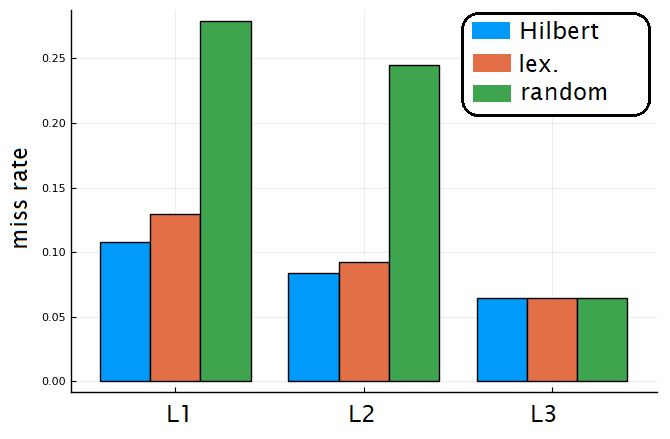
\includegraphics[width=\linewidth]{figures/missrates.png}
\caption{Cache miss rates were estimated using the cache simulator for Hilbert, lixicographic and random element orderings. Hilbert order shows the lowest miss rate. The random ordering was used to show a very bad case.}
\end{figure}

\section{Demonstrations}
Some example applications are outlined here. The focus is more toward the DSL aspect and the types of problems that this tool is designed for, rather than performance benchmarks. Since external code generation relys on the parallel capabilities of the target framework, we refer the reader to the demonstrated performance measurements of those. For example, the Dendro framework has shown competetive scalability for large scale simulations\cite{dendro}\cite{dendro2}. For \FMshop's internal performance, parallelization strategies are currently under development, and competetive benchmarks have not yet been established.

\subsection{Steady-state Advection-diffusion-reaction Equation}
The following equation(\ref{eq:adr}) was used to demonstrate the ability to easily select code generation targets and to highlight the accessability of high performance solutions. 
\begin{equation}
\label{eq:adr}
\nabla \cdot (D\nabla u) + \textbf{s} \cdot \nabla u - c u = f
\end{equation}
\[
u(x\in \partial \Omega) = 0
\]
Here all of the coefficients have constant value to simplify analysis, but are intentionally generated as functions of $(x,y,z)$ to increase computational complexity. The motivation for this is to demonstrate the performance for a more challenging problem. The function $f$ was chosen such that $u$ satisfies \ref{eq:sol}.
\begin{equation}
\label{eq:sol}
u(x,y,z) = \sin(3\pi x) \sin(2\pi y) \sin(\pi z)
\end{equation}

The weak form expression provided to \FMshop\ is
\begin{verbatim}
weakForm(u,"-D*dot(grad(u),grad(v)) + 
            dot(s, grad(u))*v - c*u*v - f*v")
\end{verbatim}

The problem was first solved internally with the Julia CG-FE target using a uniform $20\times 20\times 20$ mesh of hexahedral elements. The polynomial order was set to $p=2$, which resulted in 68921 nodal degrees of freedom. This is reasonable for sequential execution in roughly one minute on a typical laptop computer, and can be thought of as a coarse prototype.

The next step was to switch the target to Matlab while keeping the same mesh configuration. To accomplish this, only one line was added to the script: \begin{verbatim}
generateFor("target_matlab_cg.jl")
\end{verbatim}
 
After testing these coarse prototypes, a much finer version was solved using the Dendro target. Three lines in the script were modified to generate code for this target. 
\begin{verbatim}
generateFor("target_dendro_cg.jl", 
            params=(8,0.001,0.3,1e-6,500))
build_octree_with(f);
# removed: mesh(HEXMESH, elsperdim=20)
\end{verbatim}
The generated code was then compiled using the Dendro library. The resulting adaptively refined mesh produced by Dendro contained about $10.6\times 10^{6}$ nodes, that is better suited to parallel execution on a cluster. It was tested on the Notchpeak cluster at the Univeristy of Utah's CHPC using two-socket Intel XeonSP Skylake nodes with 32 cores each. For one to 32 processes, one node was used. For more processes additional nodes were added as needed. Figures 2 and 3 demonstrate that the meshing, assembly and solve portions of the computation scale well up to 256 processes. 
%Figure \ref{fig:scaling2}, however, shows that for large numbers of processes the mesh setup and other overhead become dominant and limit the optimal number of processes depeding on mesh refinement. 
As can be seen, we are able to obtain excellent weak and strong scaling using a very high level description of the problem. The ability to quickly prototype and resolve numerical issues and choices in Julia or Matlab before seamlessly transitioning to C++ and MPI is a key feature of \FMshop\ that can significantly speedup development time for complex multiphysics problems. 

\begin{figure}
\label{fig:scaling1}
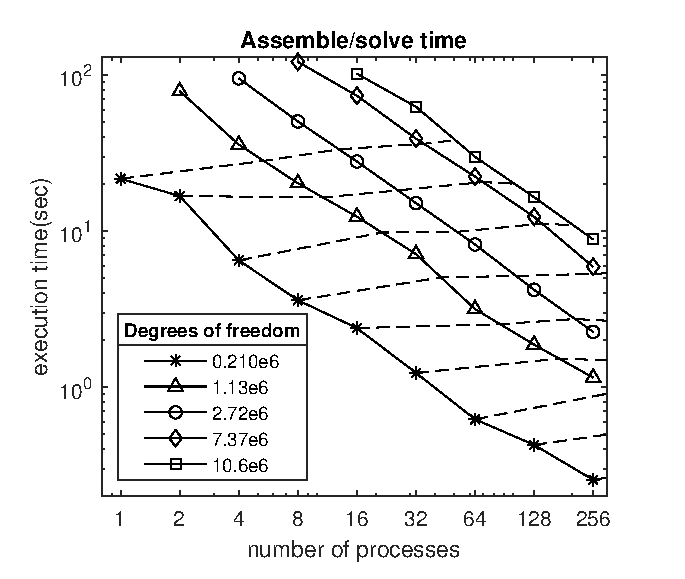
\includegraphics[width=\linewidth]{figures/solvescaling.eps}
\caption{Scaling of the assembly and solve steps. Solid lines show strong scaling for different mesh refinements(number of degrees of freedom). Dashed lines show interpolated weak scaling contours. For 1 to 32 processes, one dual socket node with 32 cores was used. For 64, 128 and 256 processes, 2, 4, and 8 similar nodes were used.}
\end{figure}
\begin{figure}
\label{fig:scaling2}
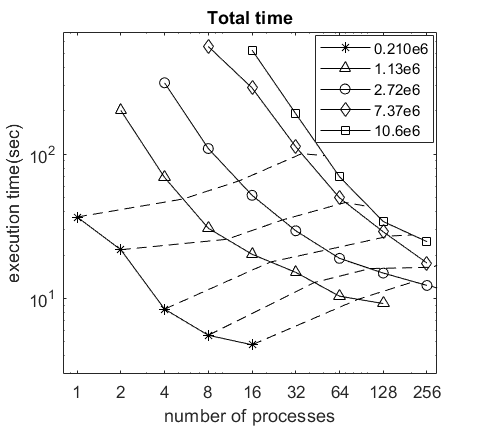
\includegraphics[width=\linewidth]{figures/totalscaling.png}
\caption{Scaling of the total execution time including mesh setup and refinement. details are similar to figure \ref{fig:scaling1}. Unlike the assembly and solve steps, the optimal number of processors for total execution time is limited depending on the mesh refinement.}
\end{figure}

\subsection{Complex Systems of PDEs}
A key principle of \FMshop\ is to simplify the translation from mathematical expressions to code. Complex systems of equations present a challenge in this respect due to the need to manage a large number of components and interactions. A good example of this is the phonon Boltzman transport equation. We refer the reader to \cite{bte2} and \cite{bte3} for the physical background and derivation of the equations. There are a number of different approaches to solving these equations. A deterministic approach that has lent itself well to parallelization is outlined in \cite{bte}, and we will adopt that formulation here. The resulting conservation-type FV equation in terms of the phonon intensity $I_{i,j}$ corresponding to directional vector $\textbf{s}_{i}$ and frequency band $\omega_{j}$ will be Eq.\ref{eq-bte}.
\begin{equation}
\label{eq-bte}
\frac{\partial \bar{I}_{i,j}}{\partial t} = \frac{1}{\tau}(\bar{I}_{0,j} - \bar{I}_{i,j}) - \frac{|v_{g}|}{V} \int_{S} I_{i,j} \textbf{s}_{i}\cdot \textbf{n} dA
\end{equation}
Where $v_{g}$, $\tau$, $I_0$ and $V$ are the group velocity, scattering time scale, equilibrium intensity, and cell volume. Integration is done over each element, or cell, and $\bar{I}$ is the cell average. The different directions are coupled through the boundary conditions via reflection as in Eq.\ref{eq-bte-bdry} with $\textbf{s}_{s}$ being the direction of specular reflection and $\alpha$ the degree of specularity.
\begin{equation}
\label{eq-bte-bdry}
I(\textbf{s}_{i}) = \alpha I(\textbf{s}_{s}) + \frac{1-\alpha}{\pi}\int_{\textbf{s}_{j}\cdot\textbf{n}<0} I(\textbf{s}_{j}) \textbf{s}_{j}\cdot\textbf{n} d\Omega_{j}
\end{equation}

The coupling between frequency bands comes from integrating over all intensities to get the equilibrium values and is done once per time step. A useful discretization may include tens of frequency bands and hundreds of directions\cite{bte}, which results in thousands of equations that are only coupled through their boundary conditions. 

To reiterate, successful parallel implementations exist for this problem, but they represent a substantial programming effort resulting in a product that would be challenging to maintain. We argue that by using FMshop this problem will be more accessible and adaptable.

For representing the quantities $I_{i,j}$ and $\textbf{s}_{i}$, where $i$ is the directional discretization and $j$ is for the frequency band, an indexed type variable will be created. As the name suggests, this is an entity that uses a single symbol, but represents an arbitrary number of components that are linked to an indexing object. This serves two purposes. First, the input expressions can then be written in terms of \texttt{I[direction, band]} and \texttt{S[direction]}, where \texttt{direction} and \texttt{band} refer to indexing objects that are involved in the assembly loops. This convenient syntax extends to other expressions such as the boundary conditions, which in this case couple all of the directions. Second, the elemental loops and loops over these indices can be transformed and different parallelization strategies can easily be applied.

The following commands illustrate how this problem could be written in \FMshop. For brevity the commands defining constants and the directional vector array have been omitted. The last command defines the loop structure with bands being the outermost loop and elements being innermost. This arrangement naturally allows working on the nearly independent bands in parallel.
\begin{verbatim}
  dir  = index("dir", range=[1,400])
  band = index("band", range=[1,40])
  I = variable("I", VAR_ARRAY, CELL, 
               index = [dir, band])
  s = coefficient("s", s_vector_array, 
               VAR_ARRAY, CELL, index = dir)

  source(I, "(Ie - I[dir,band]) / tau")
  flux(I, "vg*I[dir,band]*dot(s[dir],normal)")

  assemblyLoops(I, [band, dir, "elements"])
\end{verbatim}

To illustrate the indexed variable concept with a simpler problem, an advection equation was solved using FV for various advection speeds. The concentration variable and advection speeds both had an indexed type, so the input was simply:
\begin{verbatim}
  speed = index("speed", range=[1,5])
  u = variable("u", VAR_ARRAY, CELL, 
               index = speed)
  s = coefficient("s", s_value_array, 
               VAR_ARRAY, CELL, index = speed)
  flux(u, "upwind(s[speed],u[speed])")
\end{verbatim}
Figure 4 shows a solution to the indexed advection equation. Note the diffusion caused by the use of a first-order upwind flux.
\begin{figure}
\label{fig:advec}
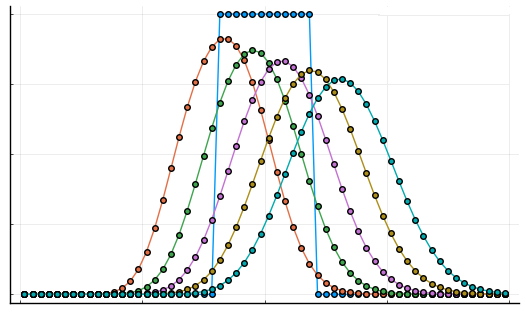
\includegraphics[width=\linewidth]{figures/addiff1dindexed.png}
\caption{Solution to advection equation for various advection speeds using indexed entities. The square pulse represents the exact solution. Note the diffusion caused by the first-order upwind flux.}
\end{figure}

\section{Conclusion and Ongoing Development}
\FMshop\ is a new and rapidly evolving toolkit that enables domain scientists to swiftly build numerical PDE solvers while taking advantage of sophisticated parallel software frameworks. It also provides an extensible resource that is designed to adapt to changes in technology, computing environment, and needs. It also adds a new set of capabilities to the Julia software ecosystem that will hopefully be adopted and expanded as new code generation targets and mathematical techniques are developed.

The list of goals and desired features is considerable, but some important ones that are either under current development or are planned for the near future include:\\
\begin{itemize}
\item Support for distributed parallelism and improved use of multithreading within \FMshop.
\item GPU utilization for suitable applications.
\item Addition of new code generation targets to provide optimal solutions for a broader range of applications and user preferances.
\item Direct use of certain external targets from within \FMshop\ to streamline the process.
\item Addition of profiling utilities to finely tune internal solution strategies.
\item Interaction with more of the great Julia libraries available to take full advantage of this scintific computing ecosystem.
\item Development of practical experiments in collaboration with domain scintists to test effectiveness and usability.
\end{itemize}

Of these items, the immediate effort will be focused on improving the internal parallel features and expanding the external generation options to make \FMshop\ competetive in terms of performance. 

The code for \FMshop, along with a set of detailed examples and usage information, can be found at https://github.com/paralab/Finch

\begin{thebibliography}{99}

\bibitem{dendro}
Milinda Fernando, David Neilsen, Hari Sundar, ``A scalable framework for Adaptive Computational General Relativity on Heterogeneous Clusters”, {\em ACM International Conference on Supercomputing, ICS’19}, 2019
\\
\bibitem{yateto}
Carsten Uphoff, Michael Bader, ``Yet Another Tensor Toolbox for Discontinuous Galerkin Methods and Other Applications", {\em ACM Trans. Math. Softw.}, vol. 46, no. 4, art. 34, 2020
\\
\bibitem{mcrae}
A. T. T. McRae, G.-T. Bercea, L. Mitchell, D. A. Ham, C. J. Cotter, ``Automated Generation and Symbolic Manipulation of Tensor Product Finite Elements", {\em SIAM J. Sci. Comput.}, vol. 38, no. 5, pp.~25--47, 2016
\\
\bibitem{homolya}
Miklós Homolya, Robert C. Kirby, David A. Ham, ``Exposing and exploiting structure: optimal code generation for high-order finite element methods", (preprint) arXiv:1711.02473, 2017
\\
\bibitem{seisol}
Ravil Dorozhinskii, Michael Bader, ``SeisSol on Distributed Multi-GPU Systems: CUDA Code Generation for the Modal Discontinuous Galerkin Method", {\em HPC Asia 2021: The International Conference on High Performance Computing in Asia-Pacific Region}, January 2021 pp.~69--82
\\
\bibitem{kempf}
Dominic Kempf, René Heß, Steffen Müthing, Peter Bastian, ``Automatic Code Generation for High-performance Discontinuous Galerkin Methods on Modern Architectures", {\em ACM Trans. Math. Softw.}, vol. 47, no. 1, art. 6, 2020
\\
\bibitem{pietro}
Daniele A. Di Pietro, Jean-Marc Gratien, Florian Häberlein, Anthony Michel, Christophe Prud'homme, ``Basic concepts to design a DSL for parallel finite volume applications: extended abstract", {\em POOSC '09: Proceedings of the 8th workshop on Parallel/High-Performance Object-Oriented Scientific Computing}, no.3, 2009
\\
\bibitem{macia}
Sandra Macià, Pedro J. Martínez-Ferrer, Sergi Mateo, Vicenç Beltran, Eduard Ayguadé, ``Assembling a High-Productivity DSL for Computational Fluid Dynamics", {\em PASC '19: Proceedings of the Platform for Advanced Scientific Computing Conference}, no. 11, 2019
\\
\bibitem{dendro2}
Milinda Fernando, David Neilsen, Hyun Lim, Eric Hirschmann, Hari Sundar, ``Massively Parallel Simulations of Binary Black Hole Intermediate-Mass-Ratio Inspirals” {\em SIAM Journal on Scientific Computing}, 2019
\\
\bibitem{bte}
Syed Ashraf Ali, Gautham Kollu, Sandip Mazumder, P. Sadayappan, Arpit Mittal,
``Large-scale parallel computation of the phonon Boltzmann Transport Equation",
{\em International Journal of Thermal Sciences}, vol. 86, pp.~341--351, 2014
\\
\bibitem{bte2}
Chang-Lin Tien, Arunava Majumdar, Frank M. Gerner (Editors), {\em Microscale Energy Transport}, Taylor
and Francis, 1998
\\
\bibitem{bte3}
Arunava Majumdar, ``Microscale Heat Conduction in Dialectric Thin Films", {\em Journal of Heat Transfer}, vol. 115, no. 1, pp.~7--16, 1993
\\
\bibitem{juliagpu}
Tim Besard, Christophe Foket, Bjorn De Sutter. ``Effective extensible programming: Unleashing Julia on GPUs." {\em IEEE Transactions on Parallel and Distributed Systems}, 2018
\\
\bibitem{pycachesim}
Julian Hammer, pycachesim: Python Cache Hierarchy Simulator, URL https://github.com/RRZE-HPC/pycachesim
\\
\bibitem{nektar}
Nektar++ URL https://www.nektar.info
\\
\bibitem{dealii}
%deal.II URL https://www.dealii.org
W. Bangerth, T. Heister, L. Heltai, G. Kanschat, M. Kronbichler, M. Maier, B. Tur-
cksin, and T. D. Young, ``The deal. II library, version 8.2", {\em Arch. Numer. Software}, vol. 3, 2015
\\
\bibitem{fenics}
%FEniCS URL https://fenicsproject.org
Martin S. Aln{\ae}s, Jan Blechta, Johan Hake, August Johansson, Benjamin Kehlet, Anders Logg, Chris Richardson, Johannes Ring, Marie E. Rognes, Garth N. Wells, ``The FEniCS Project Version 1.5", {\em Archive of Numerical Software}, vol. 3, no. 100, pp.~9--23, 2015
\\
\bibitem{firedrake}
%Firedrake URL https://www.firedrakeproject.org
Florian Rathgeber, David A. Ham, Lawrence Mitchell, Michael Lange, Fabio Luporini, Andrew T. T. Mcrae, Gheorghe-Teodor Bercea, Graham R. Markall, and Paul H. J. Kelly. ``Firedrake: automating the finite element method by composing abstractions". {\em ACM Trans. Math. Softw.}, 43(3):24:1–24:27, 2016
\\
\bibitem{openfoam}
OpenFOAM URL https://www.openfoam.com
\\
\bibitem{devito}
%Devito URL https://www.devitoproject.org
M. Louboutin, M. Lange, F. Luporini, N. Kukreja, P.A. Witte, F.J. Herrmann, P. Velesko,  G.J. Gorman, ``Devito (v3.1.0): an embedded domain-specific language for finite differences and geophysical exploration", {\em  Geoscientific Model Development}, vol. 12, no. 3, pp.~1165--1187, 2019
\\
\bibitem{diffeqjl}
DifferentialEquations.jl URL\\
https://diffeq.sciml.ai/dev/index.html
\\
\bibitem{juliabench}
Julia benchmarks URL\\
https://julialang.org/benchmarks
\\
\end{thebibliography}
\end{document}
